\section{Implementation}
\label{sec:implementation}

\begin{figure}[t]
    \centering
    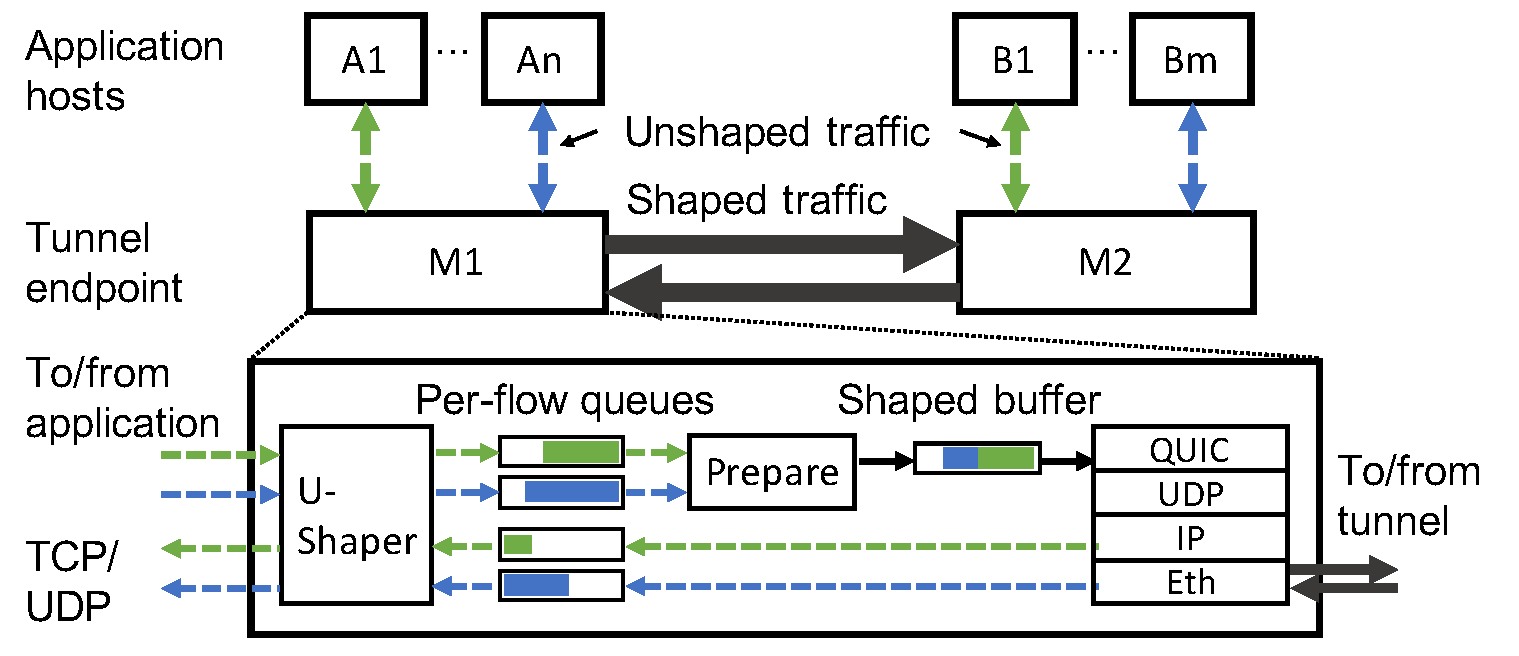
\includegraphics[width=\columnwidth]{figures/middlebox-arch.pdf}
    %    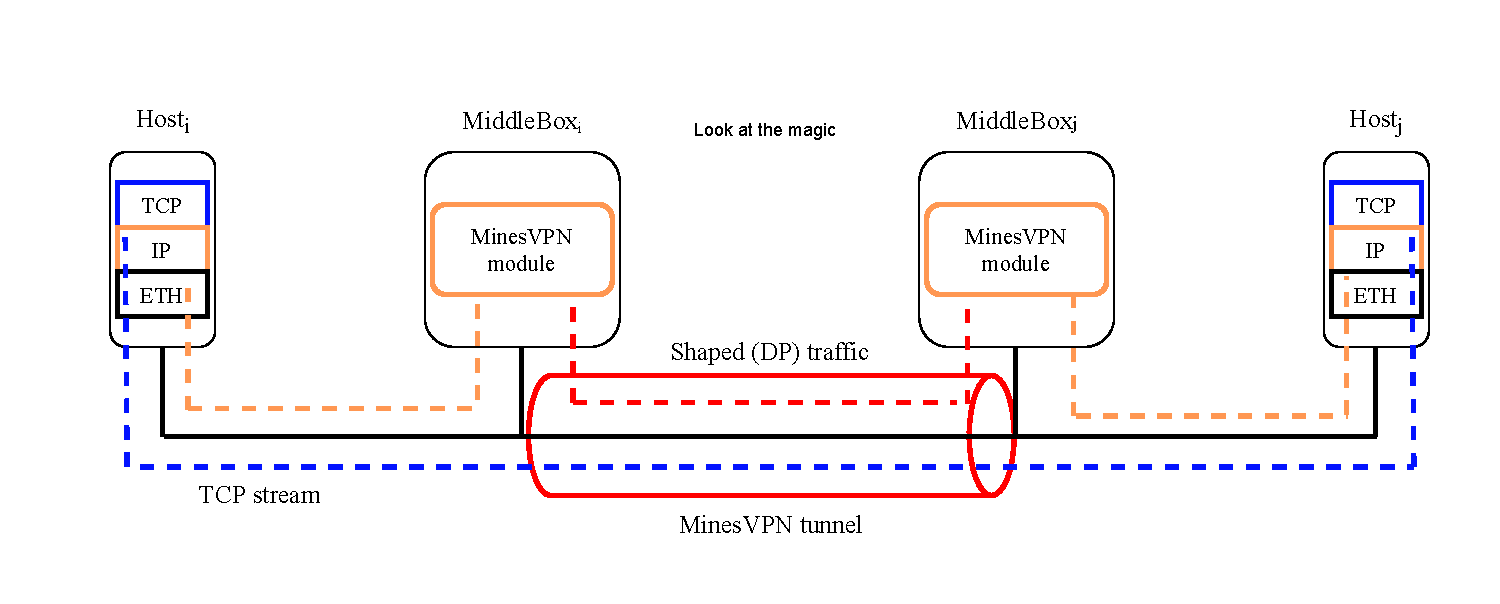
\includegraphics[width=\columnwidth]{figures/design.pdf}
    \caption{{\sys} middlebox design}
    \label{fig:minesvpn-impl}
\end{figure}

We present a middlebox based {\sys} implementation,
as shown in \Cref{fig:minesvpn-impl}.
%
Recall from \S\ref{subsec:key-ideas}, a middlebox can support shaping for
several applications and amortizes~the shaping cost among multiple flows that
share the same tunnel.
Moreover, middleboxes can support multiple ``long-term'' tunnels between
endpoints. Such tunnels may be set up, for instance, between organization
campuses to secure all communication between the campuses without the need for
modifying individual end hosts.

%\begin{table}[t]
%    \centering
%    \renewcommand{\arraystretch}{1.2}
%    \begin{tabular}{lll}
%        \toprule
%        {\bf Outer/Inner} & {\bf TCP} & {\bf UDP}
%        \\
%        \midrule
%        {\bf TCP} & meltdown & inefficient
%        \\
%        {\bf UDP} & insecure & OK
%        \\
%        \bottomrule
%    \end{tabular}
%    \caption{Impact of tunneling a transport inside transport}
%    \label{tab:transport-in-transport}
%\end{table}
%
Following the proxy architecture, the middlebox splits the communication between
two application endpoints over three transport connections:
one between two middlebox endpoints that provides a tunnel and one between
each application endpoint and its local middlebox.
In our implementation, a middlebox consists of two userspace processes,
{\ushaper} for unshaped traffic and {\dshaper} for shaped traffic,
which can run on any standard operating system kernel
and transport stack.
%For each tunnel supported by the middlebox, there is one {\dshaper} process. The
%{\ushaper} process simply multiplexes the flows mapped to all tunnels using one
%or more threads.
Together, the two processes mediate traffic between the application endpoints
and the middleboxes, and sending/receiving shaped traffic to/from the tunnel.
%{\sys}'s prototype relies on a Linux kernel with the standard TCP and UDP
%stack, and the MSQUIC implementation of the QUIC protocol.
%Together the two processes implement the following functionalities: (i)
%establishing tunnels with remote middleboxes, (ii) managing communication
%between local and remote application end points, (iii) moving traffic between
%local application endpoints and the tunnel, (iv) shaping tunnel traffic, and (v)
%providing end-to-end reliable delivery semantics.
We describe each {\sys} component and
how they ensure secret-independent shaping
both within one tunnel and then across multiple tunnels.

\if 0
\subsection{\todo{Middlebox-Middlebox Tunnel Setup}}

%Specifically, the {\dshaper} establishes tunnels with remote middleboxes, shapes
%the outbound traffic on each tunnel according to the tunnel's DP parameters, and
%handles inbound shaped traffic received from the tunnels. The {\ushaper} manages
%the connection with a local application endpoint and mediates the traffic
%between the application endpoint and the {\dshaper}.

%To protect an application's traffic, the middlebox must be placed inside the
%same private network as the application, so that the adversary cannot observe
%the traffic between an application and the middlebox.

%To establish an end-to-end connection, {\sys} relies on three piecewise
%transport connections: one between the two middlebox endpoints that provide a
%tunnel for the application endpoints, and one each between each application
%endpoint and its local middlebox endpoint.

%Each middlebox consists of two userspace processes: a {\ushaper}, which
%interfaces with the local application, and a {\dshaper}, which interfaces
%with the remote middleboxes.
%For each application flow handled by the middlebox, the {\ushaper} mediates
%establishment of the end-to-end connection between the application endpoints,
%and the sending and receiving of traffic from the associated tunnel.
%For this, the {\ushaper} maintains a set of a TCP socket, and a pair of
%transmit and receive queues.
%each application flow to its associated tunnel, sockets, and a pair of transmit
%and receive queues.

%The {\ushaper} shares with the {\dshaper} a {\flowmap} table containing
%mappings of the segments of end-to-end connections, a set of per-flow transmit
%queues, and a set of per-flow receive queues. Together, the two processes manage
%traffic flows on the end-to-end connections.

%\subsection{Shaping Components}
%{\sys} consists of two userspace processes, {\ushaper} and {\dshaper},
%which can run on top of any standard operating system and network stack. The
%{\ushaper} interfaces with the local application endpoints while the {\dshaper}
%process interfaces with the remote middleboxes of the tunnels it handles. The
%{\ushaper} shares the {\flowmap} table, a set of per-flow transmit queues,
%and a set of per-flow receive queues with the {\dshaper}.

%{\sys}'s basic proxy functionality includes setting up a connection between a
%middlebox pair that would carry shaped traffic for sensitive flows, setting up
%and tearing down a connection between the application endpoints for the
%sensitive flows, and  handling congestion. We describe these next.

%\am{de-duplicate from section 5.2, paragraph ``Traffic shaping within a
%    tunnel''.}
%For each tunnel interfacing with a remote middlebox, the {\dshaper}
%maintains a set of a QUIC socket, and a pair of threads, namely {\em Shaper}
%and {\em Shaped\-Receiver} threads.
%For each tunnel interfacing with a remote middlebox, the {\dshaper}
%maintains a set of a QUIC socket, and a pair of threads, namely {\em Shaper} and
%{\em ShapedReceiver}. The Shaper handles outbound traffic while the
%ShapedReceiver handles inbound traffic.


%\paragraph{Middlebox-middlebox tunnel setup.}
A {\sys} middlebox is statically configured with the addresses of the local
application hosts as well as other middleboxes to which the applications’
traffic must be forwarded\footnote{In practice, the middleboxes could discover
other middleboxes using DNS or similar protocols.}.
The {\dshaper} establishes QUIC tunnels with every remote middlebox specified in
its configuration.
%Each tunnel is identified by a 6-tuple consisting of the IP addresses and ports
%of source and destination middleboxes, a reliability flag, and a privacy
%descriptor.
%%{source middlebox IP, destination middlebox IP, source middlebox port,
%%destination middlebox port, reliability flag, privacy descriptor}.
%The reliability flag indicates if the tunnel provides reliable delivery
%semantics or not. The middlebox uses a reliable tunnel for shaping the traffic
%of applications using reliable transport (\eg TCP) and an unreliable tunnel for
%applications using unreliable transport (\eg UDP).
%The privacy descriptor indicates the DP configuration for the tunnel. All
%application flows passing through the same tunnel are subject to the same DP
%parameters.

After a QUIC connection is established between a pair of middleboxes, the
{\dshaper} process in each middlebox initializes three QUIC streams: a control
stream, a dummy stream, and a data stream.
%\todo{fixed number of data streams} that are used to carry the payload of
%application flows.
%The control and dummy streams are designated special stream IDs.
The control stream is used to transmit control messages related to establishment
and termination of the data stream that will subsequently transmit data in the
tunnel. The dummy stream is used to transmit padding in QUIC packets in the
form of QUIC STREAM frames.
%\am{mention reliance on QUIC's encryption protocol.}

%Once a tunnel has been established, each middlebox continuously transmits dummy
%packets at a uniform low rate in the tunnel. \am{Is it uniform as in constant
%shaping or DP shaped? How are we accounting for this overhead?}
%For this, the middlebox establishes a QUIC stream with a special ID, designated
%as the dummy stream, and generates STREAM frames of appropriate length.

\subsection{\todo{End-to-End Connection Management}}
When one application endpoint (\eg A1 in \Cref{fig:minesvpn-impl}) initiates
communication with another application endpoint (B1), the middlebox close to the
initiator (M1) and the responder (M2) work like a forward proxy and a reverse
proxy, respectively.
Together the two middlebox proxies establish a piecewise connection between the
application endpoints.

%\am{Compress to say, connection establishment like a standard forward and
%reverse proxy style.}
%Without loss of generality, we describe the the end-to-end connection
%establishment and termination in the context of a single-client-single-server
%application with one middlebox in front of each (cf.
%\Cref{fig:minesvpn-impl}).  The middleboxes in front of the client and the
%server are called the client middlebox and the server middlebox, respectively.
%
%A flow between a client and a server is carried through a connection that
%consists of three segments: (i) between the client and its middlebox, (ii)
%between the server and its middlebox, and (iii) between the client middlebox and
%the server middlebox. The {\ushaper} in the client middlebox intercepts the
%connection handshake messages from the client and notifies the {\dshaper}.
%The {\dshaper} in the client middlebox sends a handshake message to its peer
%in the server middlebox, which then notifies the {\ushaper} in the server
%middlebox. The {\ushaper} in the server middlebox initiates a handshake with
%the server on behalf of the remote client. When the handshake with the server is
%complete, the server middlebox responds to the client middlebox, which then
%completes the handshake with the client.

Once the connection is established, each application endpoint may send to the
{\ushaper} in its local middlebox an optional shaping configuration
request, which indicates the choice of DP parameters and/or latency constraints
it wishes to use for shaping its outbound
traffic\footnote{Before forwarding the DP parameters to their respective
middleboxes, the applications run an additional handshake protocol after
connection establishment to negotiate the parameters for the traffic between
them.}.
%
Finally, the {\ushaper} sets up an entry in a local {\flowmap} table to establish
shaping for the application endpoints.
%mapping the three connection segments, the associated socket and per-flow
%transmit and receive queues, and the DP parameters for traffic shaping that were
%provided by the application endpoints at the time of flow registration.
%\am{deduplicate from the overview.}

%\paragraph{End-to-end connection shutdown.}
Closing an end-to-end connection follows a similar process as connection
initiation. The {\ushaper} in each middlebox mediates the connection termination
and removes the connection entry from its {\flowmap} table.
%The {\ushaper} in a middlebox intercepts connection termination handshake
%from a client (or server); the {\dshaper} in the middlebox then relays
%connection termination to the {\dshaper} in its peer middlebox; the {\ushaper}
%process on the peer middlebox terminates connection with the corresponding
%server (or client) and responds to the initiating middlebox, which then closes
%the connection with its local node.
%Finally, both middleboxes remove the connection entry from their local
%{\flowmap} tables.
\fi

\subsection{Components}
\label{subsec:impl-mediation}
\paragraph{UShaper.}
The {\ushaper} mediates the unshaped traffic between one or more local
application endpoints and the {\dshaper} using per-flow transmit and receive
queues.
It implements a transport server (or client) for interfacing with each local
client (or server, respectively) application endpoint\footnote{The {\ushaper}
supports both UDP and TCP endpoints for applications.}.
%The type of the transport endpoint depends on the application's choice of
%transport protocol.
Additionally, it shares a {\flowmap} table with the {\dshaper},
which consists of an entry for each end-to-end flow. Each entry maps the
piecewise connections with
%the associated sockets of {\ushaper} and {\dshaper}, a
the pair of transmit and receive queues to carry the local application's byte
stream, and shaping configurations (\eg privacy descriptor) provided by an
%\todo{(\eg privacy descriptor, tunnel lifetime)} provided by an
application at the time of flow registration.
%The transmit queues of the end-to-end flows mapped to a single tunnel connection
%correspond to the tunnel's buffering queue, on which tunnel's DP guarantees
%rely.

The {\ushaper} receives the outbound traffic from a sender application
and enqueues the byte stream into a per-flow transmit queue shared with the
{\dshaper}.
It also dequeues bytes from a per-flow receive queue, repackages them
into transport packets and sends them to the receiver application.
%It also dequeues QUIC packets from a
%%the corresponding
%per-flow receive queue, discards the dummy frames, repackages the payload from
%the remaining frames into transport packets and writes them to the socket of
%the application flow.

%\if 0
\begin{figure}[t]
    \centering
%    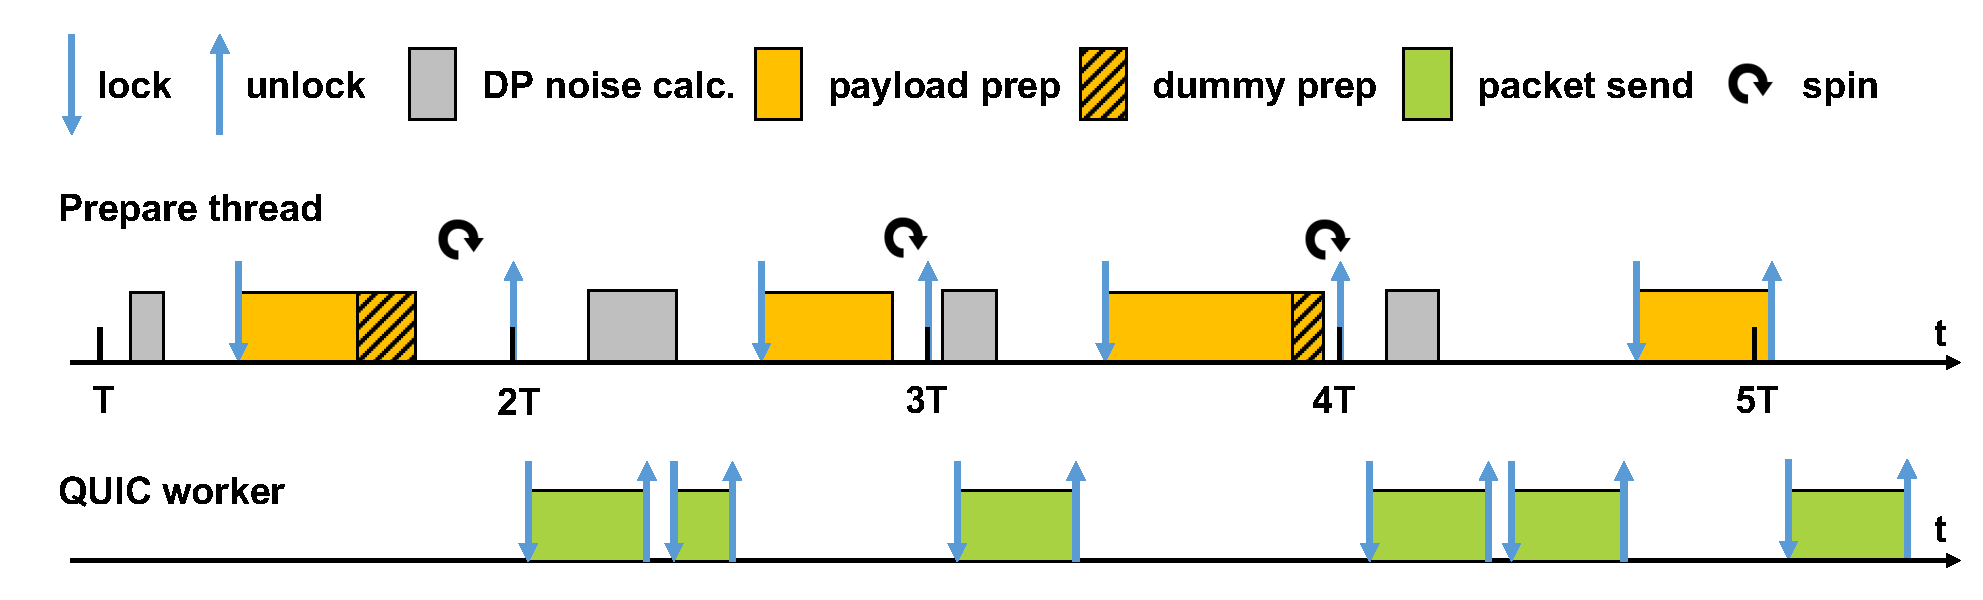
\includegraphics[width=\columnwidth]{figures/schedule.pdf}
    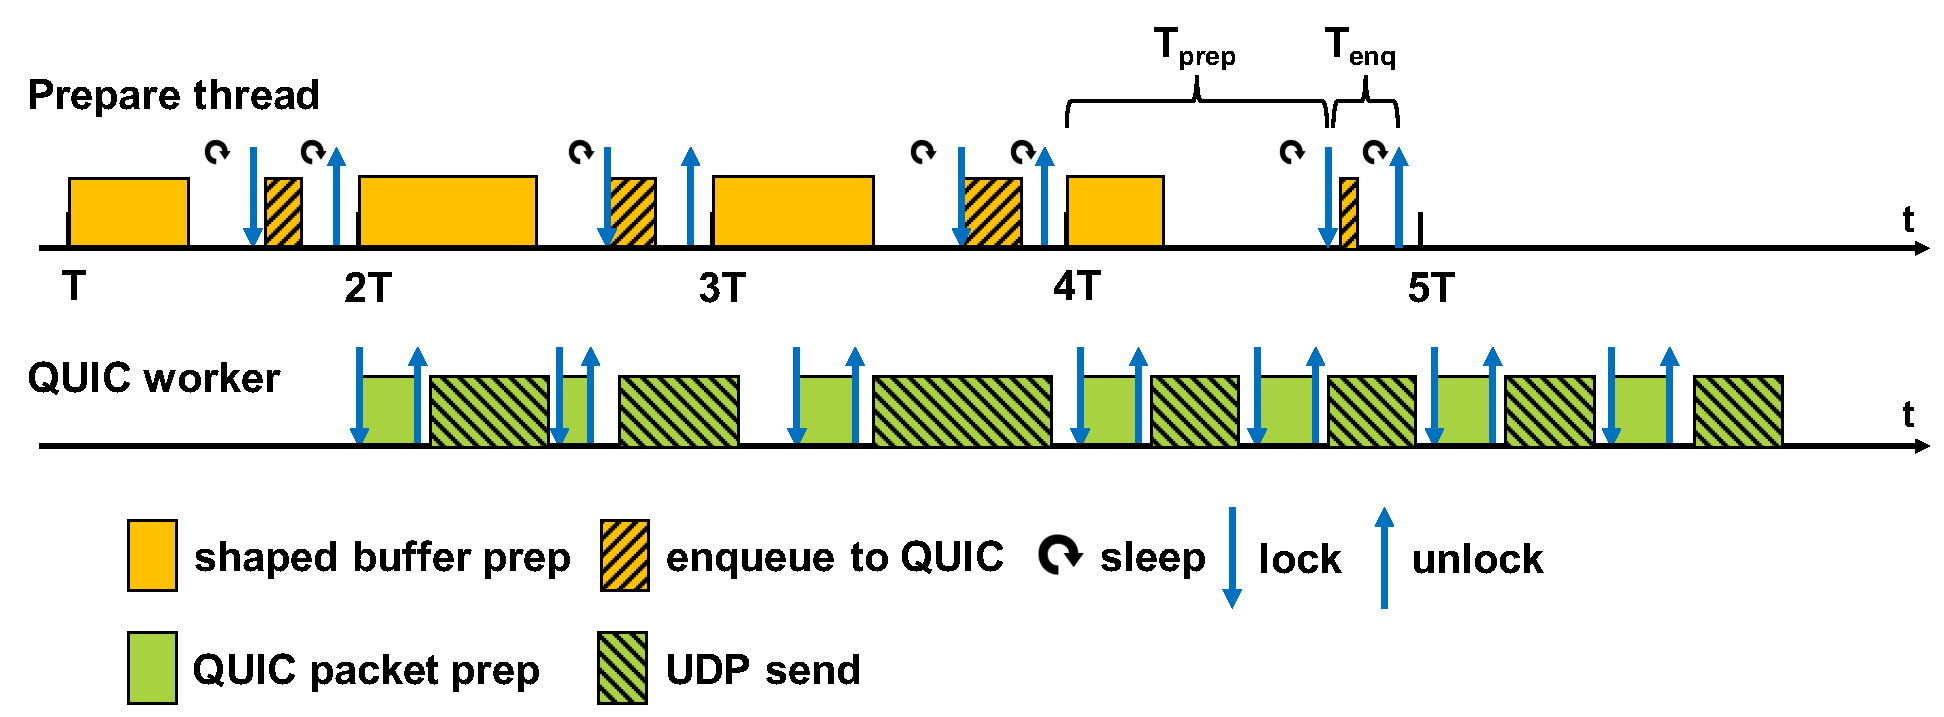
\includegraphics[width=\columnwidth]{figures/schedule5.pdf}
    \caption{{\dshaper} schedule}
    \label{fig:middlebox-schedule}
\end{figure}
%\fi

\paragraph{DShaper.}
%\label{subsec:impl-shaping}
%\am{The description does not match the security spec and will be replaced with
%the alternate text once an implementation satisfying the spec is confirmed.}
%\paragraph{Traffic shaping.}

The {\dshaper} process consists of a {\prepare} thread and a QUIC
worker thread.
The {\prepare} thread instantiates a QUIC client/server to establish
a tunnel with the remote middlebox and implements the DP shaping logic.
%On~the transmit side, {\prepare} examines the number of bytes in each
%per-flow transmit queue, determines the number of bytes to transmit,
On the transmit side, {\prepare} \update{prepares shaped buffers based on DP
measurements of the transmit queues}
and then submits shaped buffers to the QUIC worker.
On the receive size, the QUIC worker transmits ACK frames to the sender
and then decrypts the QUIC packets, extracts the STREAM frames, and copies
bytes (including dummy bytes) from each frame into the appropriate per-flow
receive queue.



%The {\dshaper} implements a thread, named {\prepare}, which instantiates a QUIC
%client/server to establish a tunnel with a remote middlebox, as well as the
%DP~shaping logic. The {\dshaper} links the QUIC library, which implements a
%worker thread that receives shaped buffers from {\prepare} and transmits them as
%one or more QUIC packets.
%\mis{I found this quite difficult to parse and want to suggest
%an alternative,
%but I was not 100\% sure that I understood the implementation well enough
%to get this right, so I'm putting it in a comment.
%The {\dshaper} process consists of a single {\prepare} thread and one
%or more QUIC worker threads.
%The {\prepare} thread both instantiates a QUIC client/serer to establish
%a tunnel with the remote middlebox and implements the DP-shaping logic.
%On the transmit side, {\prepare} examines the number of bytes in each
%per-flow transmit queue, determines the number of total bytes to transmit,
%and then submits DP-shaped buffers to the QUIC worker threads.
%On the receive size, QUIC worker threads rtansmit ACK frames to the sender
%and then decrypt the QUICK packets, extract the STREAM frames, and copy
%bytes (including dummy bytes) from each frame into the appropriateper-flow
%receive queue.
%}

%{\prepare} implements a periodic loop of length $T_{prep}$ that runs until the
%end of the tunnel lifetime.
%{\prepare} implements a while loop that runs until the end of the tunnel
%lifetime, which mainly follows the design from \S\ref{subsec:design-overview} to
%transmit shaped packets.
%After periodic intervals of length $T_{prep}$, it computes a
%differentially-private transmission size $S$ and prepares a transmit buffer of
%the same length to be sent out over QUIC.
%In each loop iteration, it prepares a transmit buffer of a
%differentially-private size $\qlendp$ to be sent to QUIC.
%{{\prepare} iterates through the transmit queues mapped to the tunnel; it
%dequeues a number of payload bytes from the queues that is the minimum of
%$\qlendp$ and the available bytes on the queues and appends them to the transmit
%buffer.}
%If the total number of payload bytes available across all transmit queues is
%lower than $\qlendp$, {\prepare} further appends dummy bytes for the remaining
%length of the transmit buffer.
%Finally, {\prepare} enqueues the transmit buffer to QUIC.

%The QUIC worker generates QUIC STREAM frames using the bytes from the
%appropriate streams passed in the transmit buffer, and then packages the STREAM
%frames into one or more QUIC packets. Finally, {the QUIC worker}
%encrypts the QUIC packet and forwards it to the underlying UDP layer, which
%ultimately transmits the packets at link speed.

%%%%%%%%%%%%%%%%%%%%%%%%%%
%%% Correct implementation
%%%%%%%%%%%%%%%%%%%%%%%%%%
%The {\dshaper} iterates through the transmit queues mapped to the tunnel; it
%dequeues a number of payload bytes from a transmit queue that is minimum of $S$
%and the available bytes on the queue, packages them into a QUIC STREAM frame,
%and appends the frame to the transmit buffer. If the total number of payload
%bytes available across all transmit queueus is lower than $S$, the {\dshaper}
%further enqueues a dummy frame of length $S - P$, where $P$ is the total number
%of payload bytes dequeued from the transmit queues. Finally, the {\dshaper}
%forwards the buffer to QUIC, which encapsulates the buffer into a QUIC packet,
%encrypts it, and then forwards it to the underlying UDP layer, which ultimately
%transmit the packet at link speed.
%At periodic intervals, the Shaper computes a differentially-private transmission
%size $S$, dequeues a number of payload bytes $P$ from the transmit queue, where
%$P$ = $min$($S$, total bytes in queue), and packages them into a QUIC frame. The
%Shaper also prepares a frame with a number of dummy bytes $D$ = $S - P$.
%Finally, the Shaper packages the payload and dummy frames into a single QUIC
%packet, encrypts the packet, and forwards the packet to the underlying UDP
%layer, which ultimately transmits the packet at link speed.

%The {\prepare} and QUIC worker threads follow the design from
%\S\ref{subsec:design-overview} to transmit shaped packets.
%When shaped QUIC packets arrive from a tunnel, QUIC transmits
%an ACK frame as a response to the sender, decrypts the received QUIC
%packets, extracts the STREAM frames, and copies the bytes (including dummy) from
%each frame into the appropriate per-flow receive queues shared with the
%{\ushaper} process.
%The {\ushaper} handles the packets as discussed in
%\S\ref{subsec:impl-mediation}.
%The {\dshaper} decrypts each inbound QUIC packet received from a tunnel and
%places
%the packet in a per-flow receive queue shared with the {\ushaper} process. QUIC
%also transmits an ACK frame as a response to the sender.
%\todo{Note that the ACK frames are themselves not subject to DP shaping.}

\if 0
%%%%%%%%%%%%%%%%%%%%
%% no longer needed?
%%%%%%%%%%%%%%%%%%%%
\paragraph{\todo{Prioritizing payload over dummy.}}
Note that %Recall that
{\prepare}'s payload preparation logic executes once at the beginning of every
interval of length $T_{prep}$.
%, \eg at time $t$, $t + T_{prep}$, $t + 2T_{prep}$, and so on.
Consider a scenario where an application's payload is
enqueued in a transmit queue at a small time $\theta$ after
the {\prepare} thread checked the transmit queue for payload bytes at the
beginning of interval $k$.
%$kT_{prep}$.
%In this case, there is no application data to transmit during the
%interval $[kT_{prep}, (k+1)T_{prep})$.
%{\prepare} will transmit dummy bytes in the interval $[kT_{prep},
%(k+1)T_{prep})$, while the application
%payload will be delayed by at least $T_{prep}$ and will be transmitted during
%the next interval $[(k+1)T_{prep}, (k+2)T_{prep})$.
{\prepare} will transmit dummy bytes in the interval $k$, while the
application payload will be delayed by at least $T_{prep}$ and will be
transmitted during the next interval ${k+1}$.
To reduce the transmission latency for the application, {\sys} modifies the
implementation of {\prepare} such that it can prioritize
payload bytes over dummy bytes more frequently.

{\prepare} implements a higher frequency loop with interval $T_{dequeue}$ inside
the
loop with interval $T_{prep}$. It splits the DP size decision generated at the
beginning of $T_{prep}$ into $T_{prep}/T_{dequeue}$ smaller uniform sizes and
prepares smaller transmit buffers by checking the transmit queue once at the
beginning of every $T_{dequeue}$ interval.
%\am{Revisit based on final design and experiments.}
\fi

%When the {\DPlogic} computes the size for the next burst transmission, it places
%a token in a local {\tokenq} rather than immediately dequeueing bytes from
%{\txq}. The packetizer, which is now decoupled from the {\DPlogic}, periodically
%checks the {\tokenq}. If the {\tokenq} is non-empty, it dequeues payload and
%dummy bytes appropriately from {\txq} to prepare a buffer of size determined by
%the first dequeued token; otherwise, the packetizer goes to sleep.
%
%The intervals of the {\DPlogic} and the packetizer determine a tradeoff between
%transmission latency for payload bytes and the bandwidth overhead due to dummy
%bytes.
%Optimally, the packetizer interval must be smaller than the {\DPlogic} interval,
%while the {\DPlogic} interval must align with the application traffic rate.
%However, the {\DPlogic} interval must not be highly reactive to the application
%traffic rate as it could reveal application secrets.
%In practice, {\sys} would incur low overheads when the traffic has a stable
%burst rate.
%%\todo{TODO}

%\paragraph{Privacy aggregation and flow prioritization.}
%{\sys} allows clients to configure the tradeoff between their individual privacy
%and overheads.
%%In principle, {\sys} provides DP guarantees individually for each application
%%flow.
%In principle, {\sys} can shape each application flow through an independent
%tunnel with per-flow DP guarantees. However, if several application endpoint
%pairs use the same middleboxes as tunnel endpoints, they can choose to amortize
%their overheads by sharing a tunnel and their DP privacy budget.
%%However, clients using the same tunnel can choose to amortize their overheads
%%by sharing their privacy budget.
%Additionally, they may provide a prioritization factor to allow {\sys} to select
%payload bytes from their per-flow queues in order of their priority. Clients can
%notify their middlebox about their desired privacy guarantee and prioritization
%factor using the privacy configuration protocol.
%
%To shape multiple flows through a shared tunnel, a {\dshaper} initializes a
%fixed
%number of data streams in the tunnel connection. When the {\ushaper} receives a
%new
%application flow, it adds a mapping for the application connection, and a pair
%of transmit and receive queues with the shared tunnel connection. Upon receiving
%a privacy configuration message, the {\ushaper} updates the configuration of a
%flow. Subsequently, at each interval, the {\dshaper} process selects payload
%bytes
%by iterating through the per-flow queues belonging to the same privacy class in
%order of the queues' priority.

\subsection{Ensuring Secret-Independent Shaping}
\label{subsec:impl-shaping-security}
%\Cref{fig:middlebox-schedule} illustrates the schedule of operations on
%{\prepare}
%and QUIC worker threads on the outbound path.
%The green and orange boxes represent data-independent and data-dependent
%operations, respectively.
The goal of the middlebox is to ensure that {\em an adversary observes
$\qlendp$ bytes in each transmit interval $\dpintvl$.}

Let's first understand the factors that might prevent the middlebox from
guaranteeing this property.
Even though an application is physically isolated from the middlebox and can
encrypt its data (\eg using end-to-end TLS), its flow control behavior could be
secret-dependent and could affect the middlebox's execution.
For instance, the presence or absence of payload traffic from an application
can affect the time {\dshaper} requires to prepare the shaped buffers.

Ensuring the high-level goal mentioned above requires that
(i) {\prepare} computes $\qlendp$, allocates and prepares a buffer of length
$\qlendp$, and passes the buffer to the QUIC worker within $\dpintvl$,
(ii) the QUIC worker prepares encrypted packets from the buffer and sends them
to UDP, such that the total payload size of the QUIC packets prepared in
$\dpintvl$ is $\qlendp$, and
(iii) the UDP stack transmits the packets totaling to $\qlendp$ bytes of payload
size to the NIC in $\dpintvl$.
Enforcing all these properties would produce a strict time-trigggered schedule
for each component, which would significantly reduce link utilization and
increase packet transmission latencies.
%Moreover, the value of $\dpintvl$ required would be large to account for
%potential secret-dependent (\eg flow control) as well as secret-independent
%delays (\eg congestion control).
%This would significantly increase packet transmission latencies.

{\dshaper} instead provides the following guarantees. (See
\Cref{fig:middlebox-schedule} for reference.)
%The {\dshaper} provides two guarantees.
First, {\prepare} \update{guarantees that a DP measurement $\qlendp$ is performed
every fixed time interval $\dpintvl$}.
Secondly, {\prepare} guarantees that a shaped buffer of length $\qlendp$ is {\em
prepared} within a fixed time $\dpintvl_{prep}$.
Thirdly, {\prepare} locks the shaped buffer for a fixed time,
$\dpintvl_{enq}$, during which it enqueues the shaped buffer for a QUIC
worker.
This ensures that the buffer is completely enqueued before QUIC starts
transmitting it and that
QUIC receives the buffer only at fixed delays.
%\todo{
We empirically profile the time taken by {\prepare} for preparing and enqueueing
shaped buffers for various DP lengths. We set $\dpintvl_{prep}$ and
$\dpintvl_{enq}$ to maximum values determined from profiling, and $\dpintvl$ to
the sum of these maximum values. If {\prepare} takes time less than
$\dpintvl_{prep}$ (or $\dpintvl_{enq}$, respectively) to prepare (or enqueue) a
shaped buffer, it sleeps until the end of the interval before moving to the next
phase.
%}
%\todo{We empirically profile the maximal time $\dpintvl^{max}_{prep}$ and
%$\dpintvl^{max}_{enq}$ taken by {\prepare} for preparing and enqueueing shaped
%buffers for various DP sizes. We set $\dpintvl_{prep} = \dpintvl^{max}_{prep}$,
%$\dpintvl_{enq} = \dpintvl^{max}_{enq}$, and $\dpintvl = \dpintvl^{max}_{prep} +
%\dpintvl^{max}_{enq}$. If {\prepare} takes time less than
%$\dpintvl^{max}_{prep}$ (or $\dpintvl^{max}_{enq}$, respectively),
%to prepare (or enqueue) a shaped buffer,
%it sleeps until the end of the interval before moving to the next
%phase.}
%\am{Too symbol heavy?}


%{\dshaper} instead provides two guarantees.
%%The {\dshaper} provides two guarantees.
%First, {\prepare} guarantees that each shaped buffer is {\em prepared} within a
%fixed time interval $\dpintvl$.
%\todo{For this, we empirically profile the maximal time taken $\dpintvl_{max}$
%by {\prepare} until
%buffer preparation for various DP sizes and set $\dpintvl$ to this
%$\dpintvl_{max}$. If {\prepare} takes lesser time than $\dpintvl_{max}$ to
%prepare a transmit buffer, it sleeps until the end of the interval, at which
%point it starts enqueueing the buffer to QUIC.}
%Secondly, QUIC's packetization remains data-independent. For this, {\prepare}
%synchronizes with the QUIC worker on the the transmit buffers,
%%the preparation of buffers to be transmitted,
%ensuring that QUIC cannot receive fewer bytes than the computed DP
%size of the interval before it sends packets to the network. F

In the middlebox, {\prepare} and QUIC worker threads run on a separate cores
sharing only the shaped buffers.
{\ushaper} runs on yet a differnet core, shares only the
{\flowmap} and the per-flow queues with {\dshaper}.
Variations in {\prepare}'s execution due to the state of the
per-flow queues are hidden by $\dpintvl_{max}$, while QUIC's
execution depends only on shaped buffers and thus, is secret-independent.
Consequently, the packetization of shaped buffers in the QUIC worker and the UDP
stack is secret-independent and any variations in packet transmit times induced
due to their execution constitute post processing noise.

A remaining concern could be leaks via internal side channels in the middlebox
that cause {\dshaper} to fail to prepare the expected amount of data within a
scheduled interval.
For instance, {\dshaper}'s execution could be influenced by microarchitectural
state (\eg caches, memory and PCI buses, write buffers, interrupts) based on the
application's flow control.

\if 0
A remaining concern could be leaks via internal side channels in the middlebox
that cause {\sys} to fail to transmit the expected amount of data within a
scheduled interval. Even though an application is physically isolated from the
middlebox and may encrypt its data (\eg using TLS for the end-to-end
connection), the application’s flow control could be secret-dependent and could
affect {\sys}'s execution.

\todo{For instance, flow control affects the number of payload bytes available
for transmission and, consequently, the amount of padding that may be added to a
segment. Processing payload and dummy bytes could take different amounts of
time.} Secondly, the execution of the Shaper could be influenced by interrupts
or microarchitectural state (\eg caches, memory and PCI buses, internal write
buffers) based on the presence or absence of payload traffic from the
application.
\fi

We have not been able to exploit such side channels to identify traffic content.
Nevertheless, such side channels could be eliminated via resource partitioning,
performance isolation, and constant-time implementation techniques
\cite{liu2016catalyst, coppens2009practical, zhang2011predinteractive,
    almeida2016verifying}.



\subsection{Scheduling Across Tunnels}
{When transmitting traffic on multiple tunnels, {\sys} must ensure that the
unshaped traffic of one tunnel is not leaked to another tunnel. For this, {\sys}
must isolate the tunnels from each other in the middlebox.
%Based on \S\ref{subsec:impl-shaping-security}, we require that the {\prepare}
%and QUIC worker threads must be performance isolated from {\ushaper} in each
%tunnel, (ii) the timing of {\prepare} must be masked to secret-independent
%times.
Thus, {\sys} partitions the middlebox cores into three groups, each core group
hosting the {\ushaper} process, the {\prepare} threads, and the QUIC worker
threads from different tunnels.
Furthermore, {\sys} uses a TDMA schedule among the {\prepare} threads, while
\update{padding} each thread's execution to a secret-independent time.
%In {\sys}, only the {\dshaper} components need to be isolated. {\sys} uses a
%TDMA to schedule the {\dshaper} processes of different tunnels.
Since each {\prepare} thread enqueues shaped buffers at secret-independent
times, the QUIC workers can subsequently package the buffers into packets and
transmit the packets across multiple tunnels following any arbitrary schedule.}
%
{Determining optimal TDMA schedules and their adaptation to the changing
number of active tunnels is left to future work.}

\if 0
%\paragraph{Shaping outbound traffic.}
\subsection{Reliable Delivery}
\am{Explain how this is relevant to security.}
Applications relying on TCP expect reliable delivery guarantees. Thus, {\sys}'s
middlebox needs to support flow control, congestion control, and loss recovery
to enable reliable delivery across the piecewise connections.

%\paragraph{Between an end host and a middlebox.}
For a connection between an end host and the middlebox, flow control, congestion
control, and loss recovery are handled by the transport layer protocol used on
the connection as usual.
%
%\paragraph{Between two middleboxes.}
For a tunnel connection, the QUIC protocol handles flow control, congestion
control, and loss recovery in
the tunnel.
%In case of congestion or packet losses on the network carrying the tunnel
%traffic,
QUIC buffers the prepared outbound packets until they are acknowledged and
retransmits unacknowledged packets in case of packet losses. The buffered
packets contain traffic whose size and timing have been shaped; therefore,
additional delays due to network congestion or packet losses only add noise to
an adversary’s observations and do not affect application’s privacy.

%\paragraph{Impact of prolonged network instability.}
In case of prolonged congestion or losses, or if the receiver is overwhelmed for
an extended period of time, QUIC's buffers in the sender middlebox may overflow
and drop packets.
The sender middlebox must then apply a back pressure on its local end hosts to
force them into slowing down their transmissions. MinesVPN’s middlebox
implements the back pressure mechanism as follows. When the {\dshaper}'s QUIC
buffer overflows, it stops dequeueing payload bytes from the per-flow transmit
queue. This causes the transmit queue to fill up and prevents the {\ushaper}
from enqueueing more bytes into the queue, which in turn causes the {\ushaper}
process to not read bytes from the TCP socket interfacing with the application.
Consequently, TCP notifies the sender of a reduction in the receive window
causing the sender to slow down transmission. Eventually, TCP's buffers may fill
up and cause TCP to drop incoming packets from the application, ultimately
notifying the sender application's TCP stack of congestion.

The system recovers from congestion once {\dshaper} receives
acknowledgements for transmitted packets and can dequeue payload
bytes from the transmit queues\footnote{{\sys} could expedite congestion
notification to the sender application by using mechanisms, such as explicit
congestion notification \cite{ecn}. We leave a detailed analysis of congestion
handling to future work.}.

A remaining challenge arises when a sender middlebox acknowledged payload bytes
from the local sender application, but is forced to drop the bytes due to
instability on the tunnel network. This violates the reliable delivery semantics
expected by the application. Note that existing proxies face a similar challenge
too. {\sys} does not aggravate the issue and, therefore, similar to other
proxies, leaves the resolution to the application and the user.
%\am{Dealing with bytes acknowledged by middlebox but no longer able to buffer.}
%\todo{Recovery from congestion.}
\fi

%\subsection{Scheduling across tunnels.}
%Once the traffic within each tunnel is shaped, sending and receiving traffic
%across multiple tunnels can follow any schedule.





%%%%%
%%%%%
\if 0
The middlebox consists of two VMs: host-facing ({\unshapedVM}) and
tunnel-facing ({\shapedVM}). Each VM hosts a separate network stack, which
consists of a transport layer on top of a
network layer on a top of an ethernet layer. The {\unshapedVM} supports one or
more transport protocols, such as TCP, UDP, and QUIC.
The {\shapedVM} primarily relies on UDP but additionally runs three layers atop
UDP: a {\DPlogic} on top of an encryption layer, which is integrated with the
QUIC protocol~\cite{langley2017quic}\footnote{In principle, the {\shapedVM} could use
TCP as a
    reliable tunnel transport; however, we choose QUIC for \todo{reasons of efficiency and
        ease of implementation}.}.
%because it enables efficient multiplexing of multiple client streams, avoids
%head-of-line blocking,

The {\unshapedVM} receives unshaped traffic from an
end-host application and forwards it to the {\shapedVM}. The {\DPlogic} shapes
the traffic according to DP and transmits it over a QUIC connection. In the
reverse direction, the {\shapedVM} forwards the traffic received over the QUIC
connection to
the {\unshapedVM}, which in turn forwards it to the target application after
decryption and removing any padding.

We now elaborate on the interaction between an end-host application and a
middlebox, as well as the components of the middlebox.

\subsection{\unshapedVM}
%
%The {\unshapedVM} places an application's outbound bytes, including handshake
%and control packets, in the transmit queue, which are dequeued and shaped in the
%{\shapedVM}. Similarly, the {\shapedVM} places inbound packets from the tunnel
%in the receive queue, which are dequeued in the {\unshapedVM}, decrypted,
%stripped of padding, and forwarded to the appropriate end-host application.

The {\unshapedVM} contains a userspace application,
called the {\mediator}, and a small kernel module, which interact via another
FIFO queue in a shared memory region.
The kernel module maintains the {\flowmap}, which consists of the
mapping of the segments of each end-to-end connection and other configuration
parameters for the connection.
In addition, the {\mediator} interfaces with the {\shapedVM} via statically sized lockfree FIFO
queues. For each end-to-end connection, there is a pair of transmit and receive
queues allocated in a shared memory region between the VMs.

When the middlebox receives a new flow from an end host application, the kernel
module in the {\unshapedVM} intercepts the handshake messages, copies them into
the FIFO queue shared with the {\mediator} and responds to the end host in
accordance with the transport protocol.  The {\mediator} forwards the handshake
messages to the {\shapedVM}, which handles the remaining stages of the
end-to-end connection establishment with the remote peer and returns information
of the later connection segments to the {\mediator}. The {\mediator} forwards
the connection information to the kernel module, which then populates a
{\flowmap} entry for the end-to-end connection.

Once a connection is established, the kernel module also intercepts the data
packets of the end host's transport protocol, copies them into the FIFO queue
shared with the {\mediator}, and sends appropriate responses to the end host in
accordance with the transport protocol.
Furthermore, the {\mediator} decrypts packets from the receive queue, strips off
any padding, and forwards the payload bytes to the kernel module. The kernel
module encapsulates the payload with protocol headers and forwards
the packets to the appropriate end hosts.

\subsection{\shapedVM}
The {\shapedVM} implements the core of {\sys}'s traffic shaping design.
The {\shapedVM} establishes a bidirectional QUIC connection with the
{\shapedVM} in each of its peer middleboxes. Within each connection, the
{\shapedVM} further opens a \todo{bidirectional} QUIC stream with its peer,
which is assigned the stream ID 0 and is used as a stream for dummy byte
transmissions.
\todo{TODO: Complete the section}
\fi

%\begin{figure*}[t]
%\center{
    %%    \centering
    %    \subfigure[Time line of connection establishment in {\sys}] {
        %%    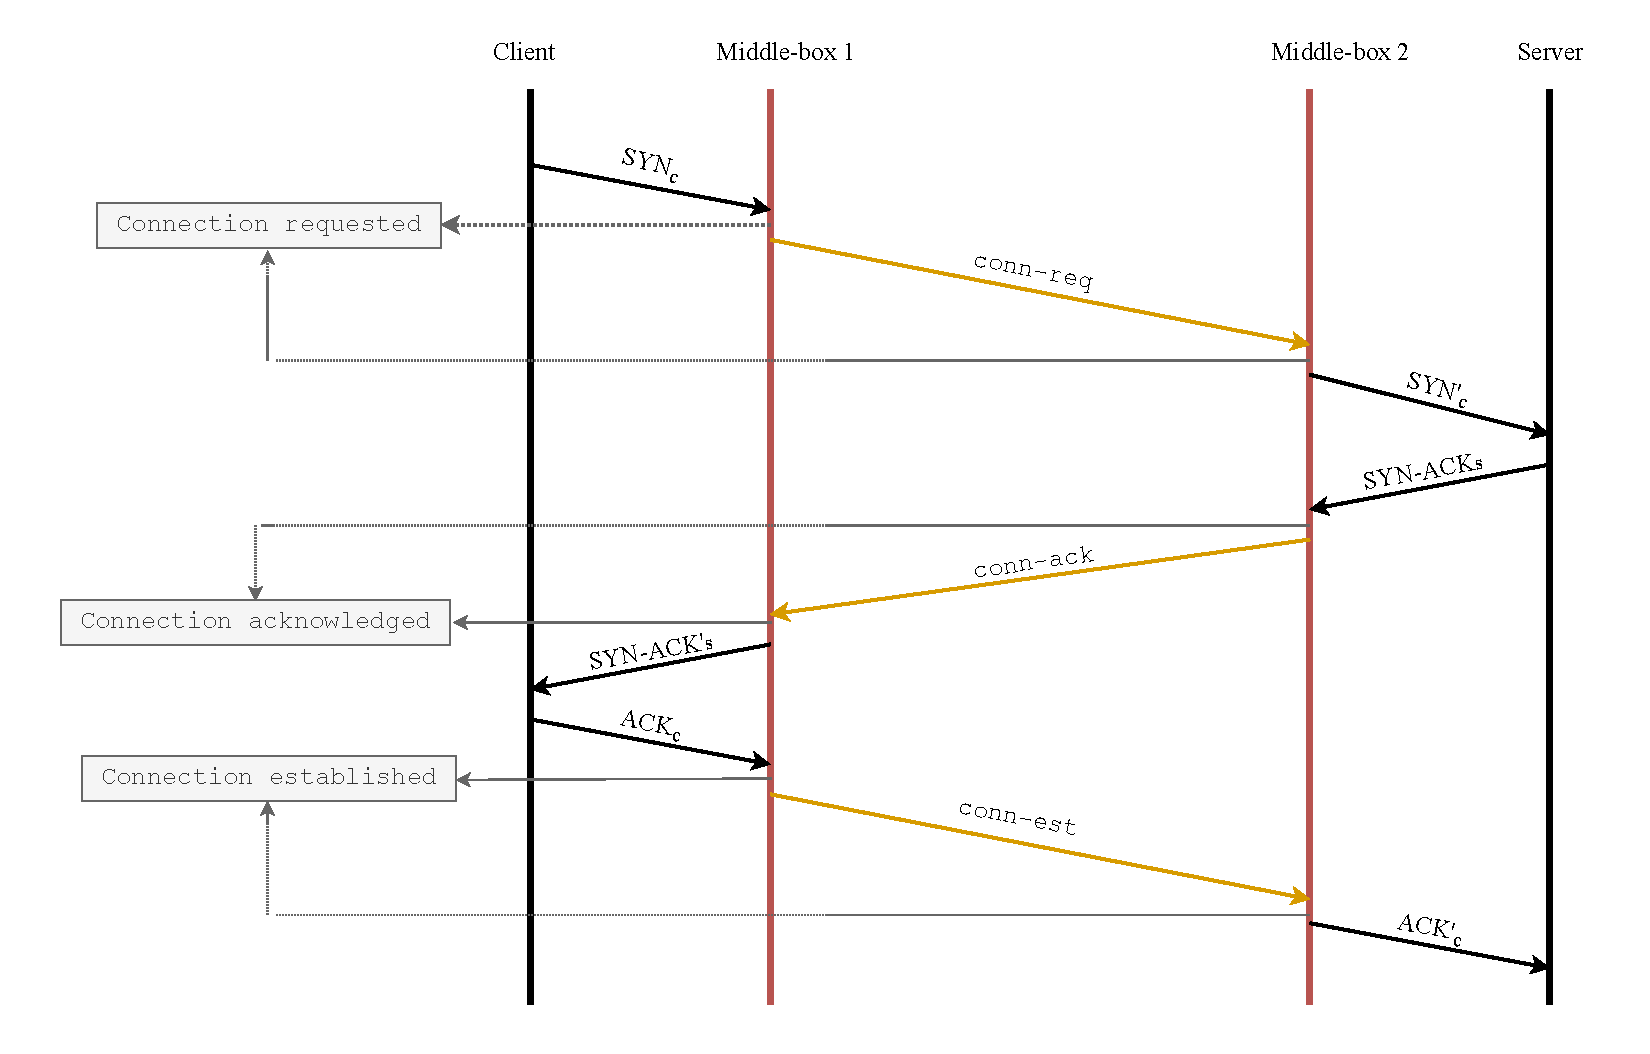
\includegraphics[width=\columnwidth]{figures/connection-establishment.pdf}
        %    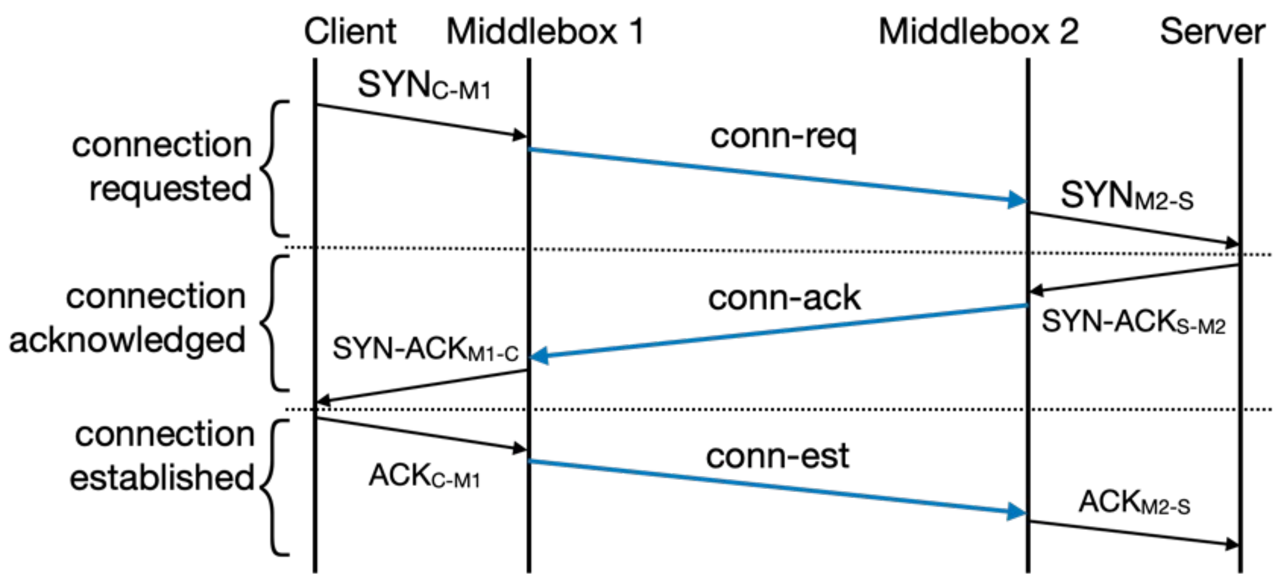
\includegraphics[width=\columnwidth]{figures/conn-est.pdf}
        %    \label{fig:connection}
        %    }
    %%\end{figure}
    %%\begin{figure}[t]
    %%    \centering
    %    \subfigure[Time line of connection termination in {\sys}] {
        %%    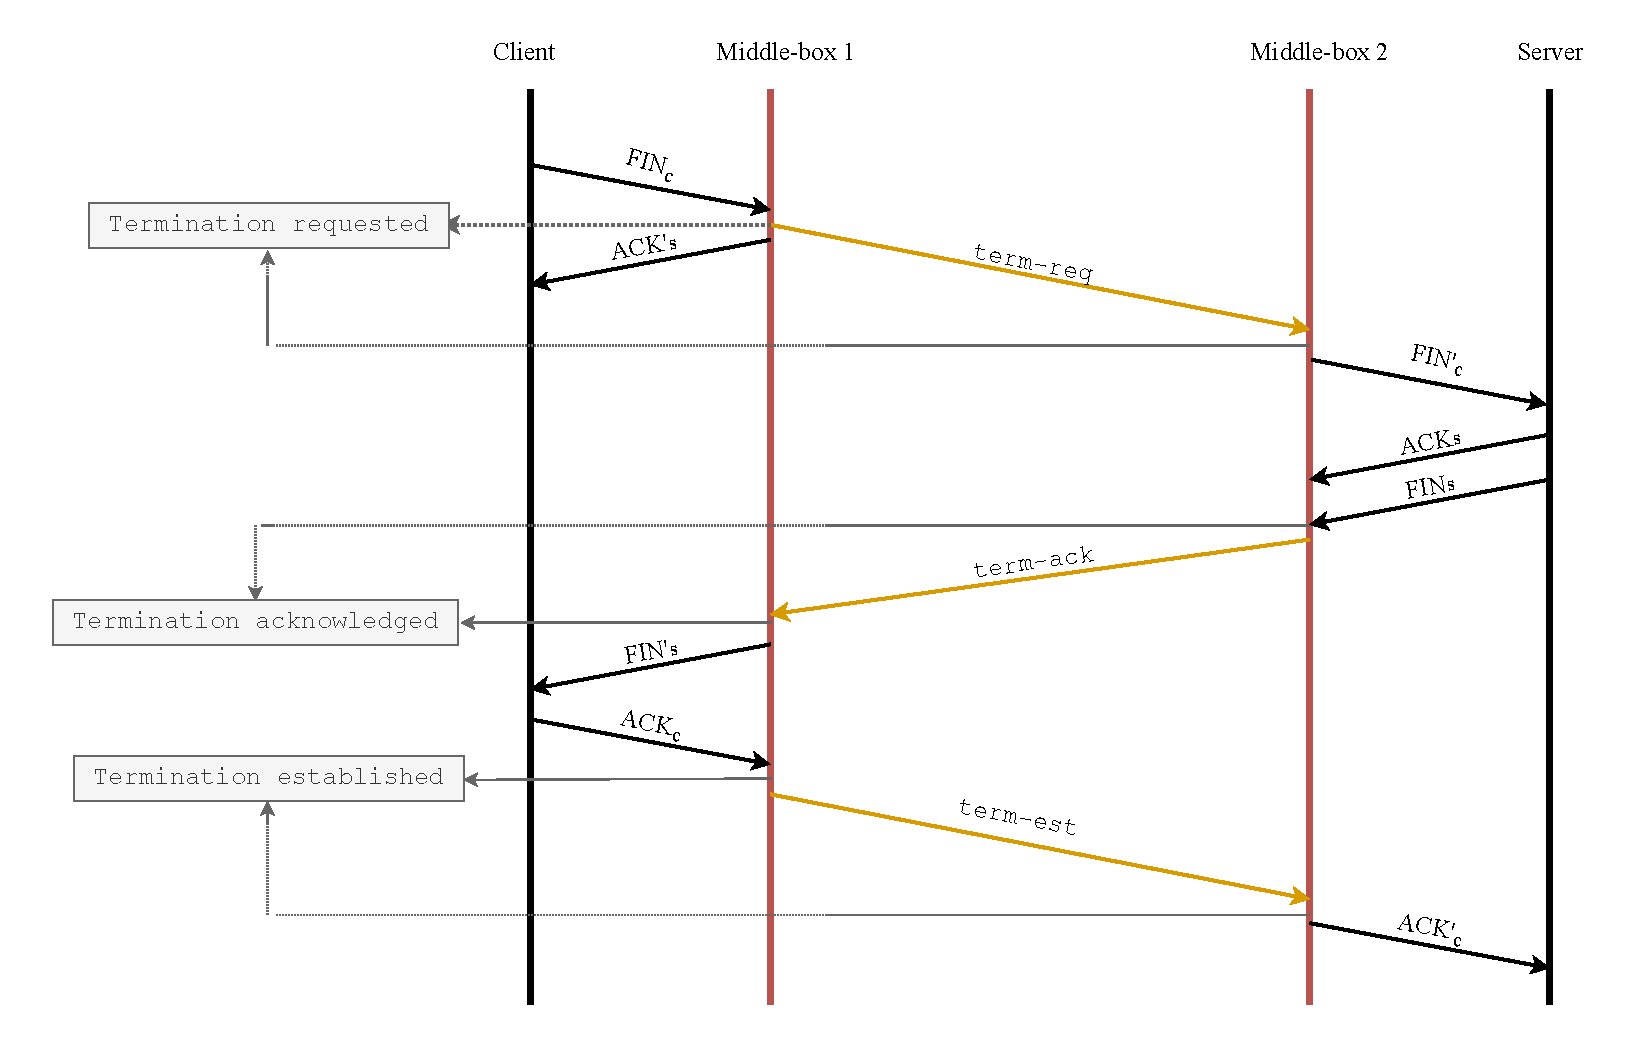
\includegraphics[width=\columnwidth]{figures/connection_termination.pdf}
        %    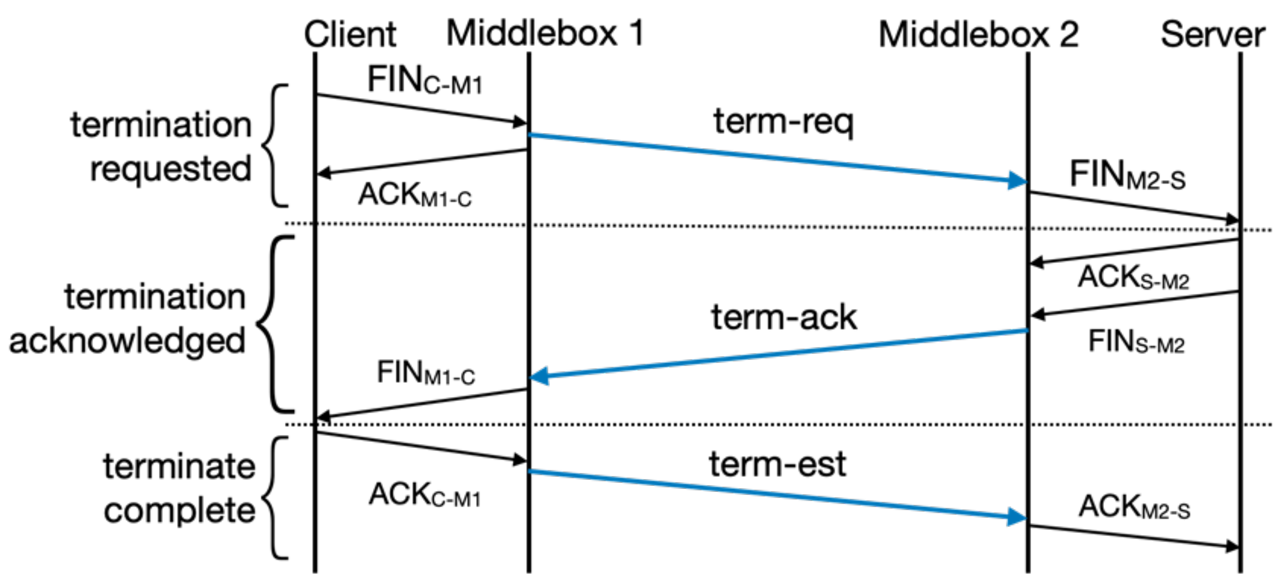
\includegraphics[width=\columnwidth]{figures/conn-term.pdf}
        %    \label{fig:termination}
        %    }
    %}
%\caption{Foo}
%\end{figure*}
%
